\subsection{Visualization}

The results of the system is visualized in rviz, which is a 3D visualization tool for ROS. 

\subsubsection{Robot}
The data published by the controller in JOINT\_STATES are the radial position of the joints. The warehouse\_viewer will use these states transformed into the coor The URDF file specifies the links between the robot’s joints and the mesh files (.stl) and tf will contain the transformations between the joints which are used in warehouse\_viewer to create 3D model of the robot. 

\begin{figure}[H]
\begin{center}
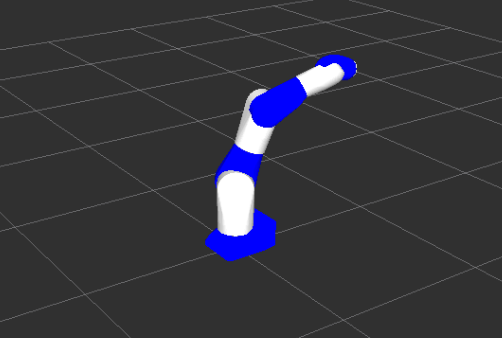
\includegraphics[width=12 cm]{robot}
\caption{3D-model of robot}
\label{tracking}
\end{center}
\end{figure}

\subsubsection{Objects}
The objects in the image that the tracking algorithm considers being real moving objects are visualized. They are published as point clouds so that rviz can subscribe them and visualize them. If the tracking algorithm believes that an object has disappeared because of non-movement, it publishes the last seen point cloud of the object i.e. static objects in the scene are objects that the system thinks are standing still. 

\begin{figure}[H]
\begin{center}
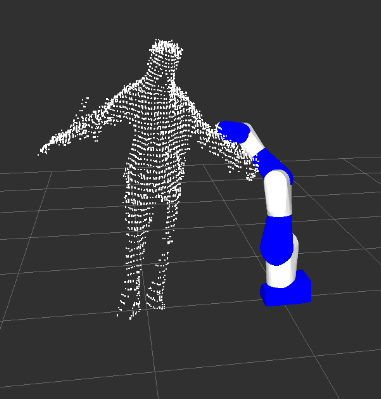
\includegraphics[width=12 cm]{humanandrobot}
\caption{3D-model of robot}
\label{tracking}
\end{center}
\end{figure}

\begin{figure}[H]
\begin{center}
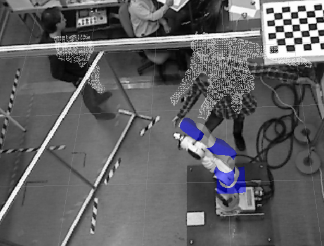
\includegraphics[width=12 cm]{humanandrobotinworld2}
\caption{3D-model of robot}
\label{tracking}
\end{center}
\end{figure}  

\subsubsection{Distances}
To visualize the resulting state of the system (the current safety zone) a line between the closest object and the closest joint of the robot visualized. This line switches color depending on which state the system is in. The color of the line is thereby the result of the system. 

//lägg in en bild på hela systemet

